\documentclass[authoryear, 12pt,5p, times]{elsarticle}
\usepackage[hypcap]{caption}
\usepackage{float}
\usepackage{amsmath}
\usepackage[hidelinks]{hyperref} 
 \usepackage{gensymb}
\usepackage{subcaption}
\usepackage{url}
%\renewcommand\thefootnote{\fnsymbol{\dagger}}
\usepackage[symbol*]{footmisc}
\begin{document}
%\footnote{This is a footnote}
\begin{frontmatter}
\title{Photon Counting \& the Statistics of Light}
\author{\today \\ \quad \\Jung Lin (Doris) Lee\\ dorislee@berkeley.edu\\Group partners: Jennifer Ito, Manuel Silvia\\Prof. James Graham, UGSI Heechan Yuk, Isaac Domagalski}
	\begin{abstract}
    %key objective, method, principle conclusion 
	ABSTRACT HERE
	\end{abstract}
\end{frontmatter}
\section{Introduction\label{intro}}
is a result of each CCD pixel's different sensitivity to photon
\begin{figure}
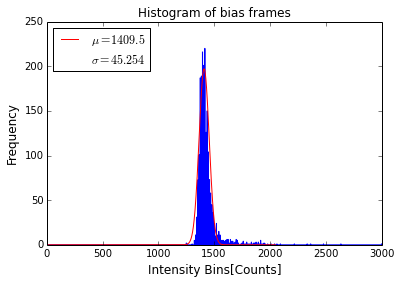
\includegraphics[width=0.5\textwidth]{figures/bias_histo}
\caption{We took a dataset of 1s integration time bias frames by placing the red cap on the spectrometer and in a black bag. A histogram of dark counts is fitted to a Gaussian. The variance of the distribution relates to the read noise and gain of the spectrometer \citep{ccd_handbook}.}
\end{figure}
\section{Conclusion}

Possible extension to this project may be to try conducting a basic flat-field correction to the detector. One way to do this to shine bright light uniformly on the detector to see the response of each pixel.  The exposure time needs to be short so that the CCD is not saturated. We can also try to measure maximum ranges at which CCD is sensitive and linear.
\bibliography{references}
 %\bibliographystyle{abbrvnat}
%\bibliographystyle{apalike}
%\bibliographystyle{plainnat}
%\bibliographystyle{unsrtnat}
\bibliographystyle{elsarticle-harv}
\end{document}
